%
\documentclass{article} % For LaTeX2e
\usepackage{iclr2021_conference,times}

% Optional math commands from https://github.com/goodfeli/dlbook_notation.
\input{math_commands.tex}

\usepackage{xcolor}
\usepackage[activate={true,nocompatibility},final,tracking=true,kerning=true,factor=1100,stretch=10,shrink=10]{microtype}
\setlength{\marginparwidth}{2cm}
\usepackage[colorinlistoftodos]{todonotes}
\usepackage{enumitem}
\usepackage{bbm}
\usepackage{natbib}
\usepackage{amsfonts}
\usepackage{amssymb}
\usepackage{amsmath}
\usepackage{graphicx}% Include figure files
\usepackage{dcolumn}% Align table columns on decimal point
\usepackage{bm}% bold math
\usepackage[ruled, vlined]{algorithm2e}
\usepackage{subcaption}
\usepackage{tikz}
\usetikzlibrary{positioning,arrows}

\usepackage[unicode,linktocpage=true,breaklinks]{hyperref}% add hypertext capabilities
\hypersetup{
  colorlinks=true,
  urlcolor=green,
  linkcolor=magenta,
  citecolor=cyan,
}

\definecolor{blue1}{HTML}{448aff}
\definecolor{pink1}{HTML}{FA5477}

\title{Neural Transformations for \\Efficient Topological Mixing}% in Lattice Gauge Theory}

% Authors must not appear in the submitted version. They should be hidden
% as long as the \iclrfinalcopy macro remains commented out below.
% Non-anonymous submissions will be rejected without review.

\author{Sam Foreman, Xiao-Yong Jin\& James Osborn\thanks{\hyperref{%
      https://github.com/saforem2/l2hmc-qcd
   }{https://github.com/saforem2/l2hmc-qcd} \\
   Leadership Computing Facility\\
   Argonne National Laboratory\\
   Lemont, IL 60439
   \texttt{\{foremans,xjin,\}@anl.gov},%
   \texttt{\{osborn\}@alcf.anl.gov}\\
}}

% The \author macro works with any number of authors. There are two commands
% used to separate the names and addresses of multiple authors: \And and \AND.
%
% Using \And between authors leaves it to \LaTeX{} to determine where to break
% the lines. Using \AND forces a linebreak at that point. So, if \LaTeX{}
% puts 3 of 4 authors names on the first line, and the last on the second
% line, try using \AND instead of \And before the third author name.

\newcommand{\fix}{\marginpar{FIX}}
\newcommand{\new}{\marginpar{NEW}}

% \iclrfinalcopy % Uncomment for camera-ready version, but NOT for submission.
\begin{document}


\maketitle

\begin{abstract}
   We propose a generalized version of the L2HMC algorithm~\citep{levy2017}, and evaluate its ability to sample from
   different topologies in a two-dimensional lattice gauge theory.
   %
   In particular, we demonstrate that our model is able to successfully mix between modes of different topology,
   significantly reducing the computational cost required to generate independent gauge configurations.
\end{abstract}

\section{Introduction}
%
Hamiltonian Monte Carlo
\begin{figure}[htpb]
   \centering
   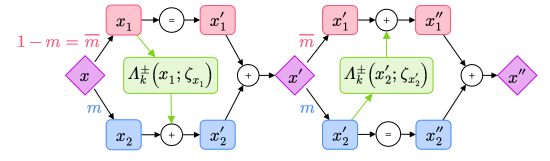
\includegraphics[width=\textwidth]{figures/splitx.pdf}
   \caption{\label{fig:split_x}Illustration of the split \(x\) update.}
\end{figure}
%

\subsubsection*{Acknowledgments}
This research used resources of the argonne leadership computing facility, which is a doe office of science user
facility supported under contract DE\_AC02--06CH11357.%
%
This work describes objective technical results and analysis.
%
Any subjective views or opinions that might be expressed in the work do not necessarily represent the views of the u.s.
doe or the united states government.

% Use unnumbered third level headings for the acknowledgments. All
% acknowledgments, including those to funding agencies, go at the end of the paper.


\bibliography{main}
\bibliographystyle{iclr2021_conference}

\appendix
\section{Appendix}
You may include other additional sections here.

\end{document}
